\documentclass{report}
\usepackage{polski}
\usepackage[utf8]{inputenc}
\usepackage{float}
\usepackage{graphicx}
\usepackage{caption}
\usepackage{subcaption}
\usepackage{ragged2e}
\usepackage{blindtext}
\usepackage{hyperref}
\graphicspath{ {../plots/} }
\begin{document}
\author{Jakub Ogrodowczyk}
\AddToHook{cmd/section/before}{\clearpage}


\section*{Moment pierwszej kolizji \((B_n)\)}
\justifying
Moment pierwszej kolizji to punkt w naszej symulacji gdy jakiś kubeł został wybrany
po raz drugi. Jest to wariacja problemu Birthday Paradox, który opisuje szansę na to,
że dwie osoby w m-osobowej grupie mają urodziny w ten sam dzień.
Paradoks polega na tym, że szansa na to aby dwie osoby współdzieliły dzień urodzin
wynosi 50\% już dla tylko 23 osób. Zmienna \(B_n\) symuluje birthday paradox dla \(n=365\)
co widzimy także na wykresie (dla n tak dużego jak 100000 potrzebujemy średnio
 zaledwie około 400 prób). Na wykresie widzimy, że koncentracja wokół średniej jest
 dość niska oraz rośnie wraz z \(n\).
    \begin{figure}[htp]
        \centering
        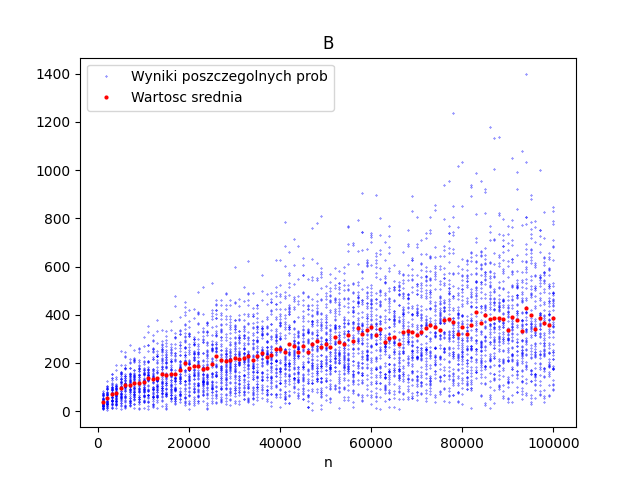
\includegraphics[scale=0.7]{plotB.png}
        \caption[Example .]{Wykres przedstawiający wyniki poszczególnych eksperymentów oraz wartość średnią \(B_{n}\)}
        \label{plotB}
    \end{figure}
    
    \clearpage

    \begin{figure}[H]
        \centering
        \begin{subfigure}{.5\textwidth}
          \centering
          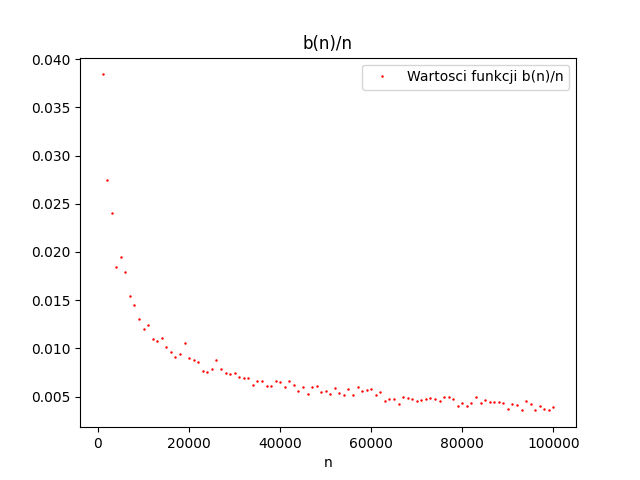
\includegraphics[width=1.1\linewidth]{plotbnfunc1.png}
          \caption{\( \frac{B_n}{n} \)}
          \label{fig:plotbnfunc1}
        \end{subfigure}%
        \begin{subfigure}{.5\textwidth}
          \centering
          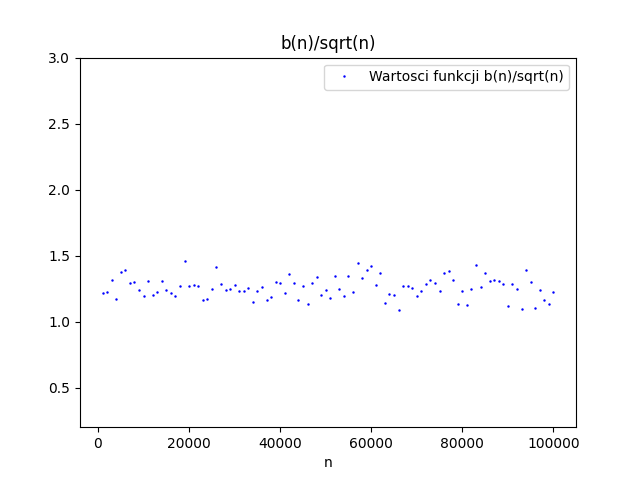
\includegraphics[width=1.1\linewidth]{plotbnfunc2.png}
          \caption{\( \frac{B_n}{\sqrt{n}} \)}
          \label{fig:plotbnfunc2}
        \end{subfigure}
        \caption{Wykresy pomagające w znalezieniu asymptotyki funkcji \(B_n\)}
        \label{fig:bn}
    \end{figure}
\center{Hipoteza:}
\[B_n=O(\sqrt{n})\]


\section*{Liczba pustych urn po wrzuceniu n kul \((U_n)\)}
\justifying
Ilość pustych urn po wrzuceniu n kul.
Obserwacje są silnie skoncentrowane wokół wartości średniej, ponadto
ich koncentracja nie rośnie wraz z \(n\).
    \begin{figure}[htp]
        \centering
        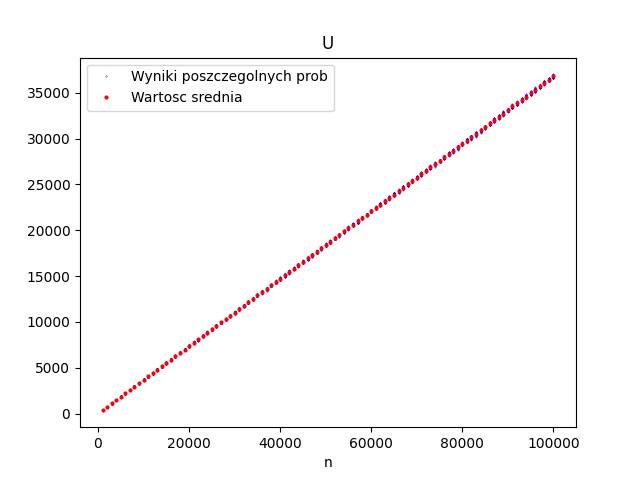
\includegraphics[scale=0.7]{plotU.png}
        \caption[Example .]{Wykres przedstawiający wyniki poszczególnych eksperymentów oraz wartość średnią \(U_{n}\)}
        \label{plotU}
    \end{figure}

    \begin{figure}[H]
        \centering
        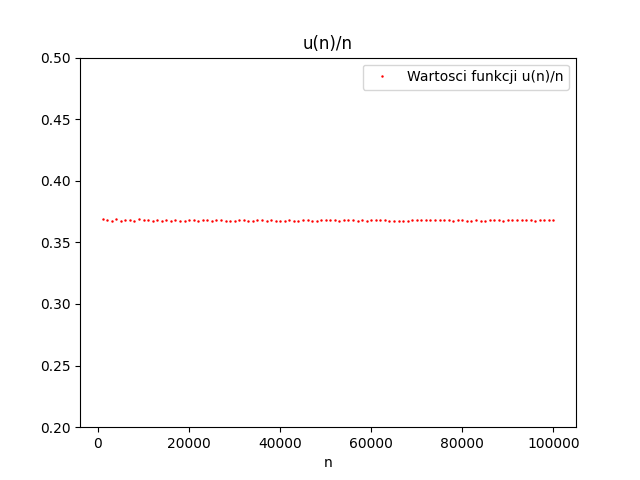
\includegraphics[scale=0.7]{plotunfunc.png}
        \caption[Example .]{Wykres pomagający w znalezieniu asymptotyki funkcji \(U_n\)}
        \label{plotUn}
    \end{figure}
\center{Hipoteza:}
\[U_n=O(n)\]



\section*{Maximum load \((L_n)\)}
\justifying
Obserwacje są względnie silnie skoncentrowane wokół wartości średniej,
nie odbiegają one od niej o więcej niż 4 i zamykają w przedziale \([4,11]\).
    \begin{figure}[htp]
        \centering
        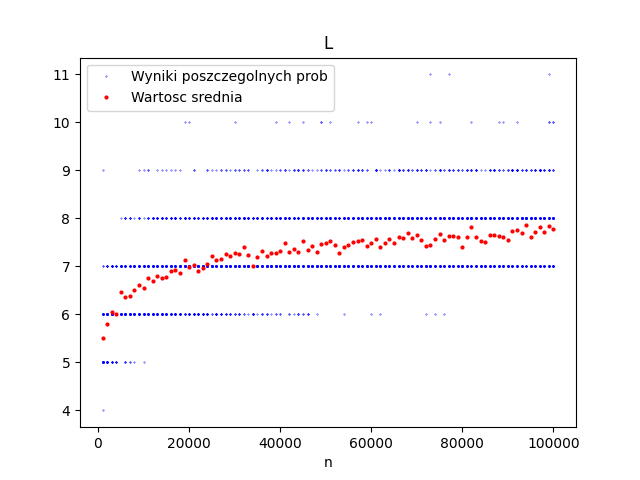
\includegraphics[scale=0.7]{plotL.png}
        \caption[Example .]{Wykres przedstawiający wyniki poszczególnych eksperymentów oraz wartość średnią \(L_{n}\)}
        \label{plotL}
    \end{figure}

    \begin{figure}[H]
        \centering
        \begin{subfigure}{.5\textwidth}
          \centering
          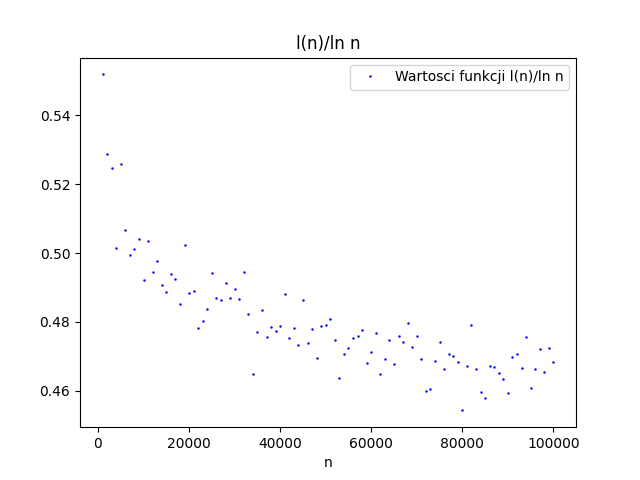
\includegraphics[width=1.1\linewidth]{plotlnfunc1.png}
          \caption{\( \frac{L_n}{ln(n)} \)}
          \label{fig:plotlnfunc1}
        \end{subfigure}%
        \begin{subfigure}{.5\textwidth}
          \centering
          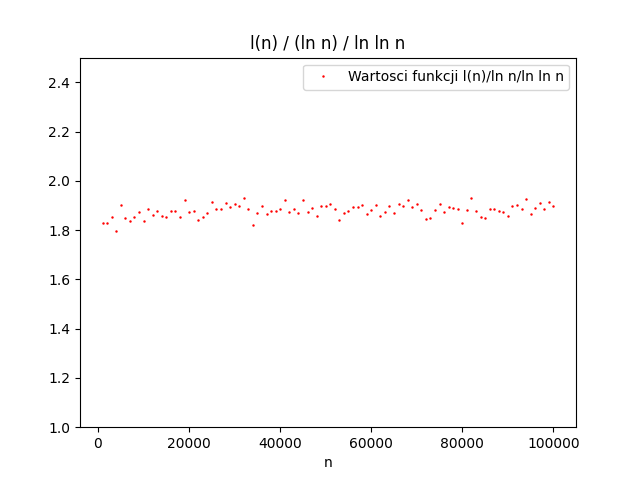
\includegraphics[width=1.1\linewidth]{plotlnfunc2.png}
          \caption{\( \frac{L_n}{\frac{ln(n)}{ln(ln(n))}} \)}
          \label{fig:plotlnfunc2}
        \end{subfigure}
        \begin{subfigure}{.5\textwidth}
            \centering
            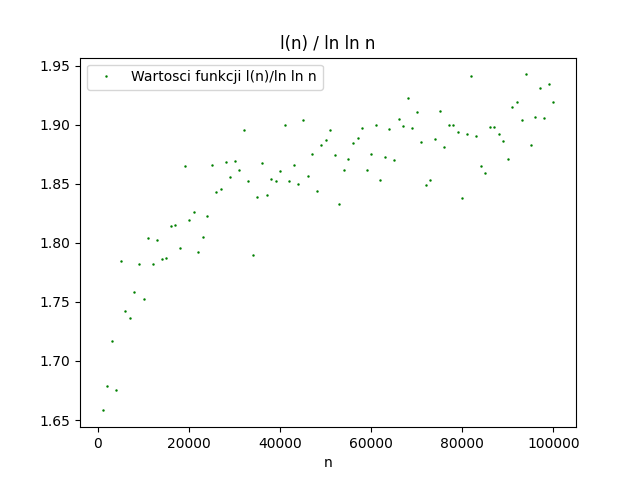
\includegraphics[width=1.2\linewidth]{plotlnfunc3.png}
            \caption{\( \frac{L_n}{ln(ln(n))} \)}
            \label{fig:plotlnfunc3}
          \end{subfigure}
        \caption{Wykresy pomagające w znalezieniu asymptotyki funkcji \(L_n\)}
        \label{fig:ln}
    \end{figure}

\center{Hipoteza:}
\[L_n=O(\frac{ln(n)}{ln(ln(n))})\]



\section*{Pierwszy moment, po którym nie ma już pustych urn \((C_n)\)}
\justifying
Minimalna liczba rzutów, po której w każdej z urn jest co najmniej jedna kula.
Zmienna ta modeluje Coupon collector's problem, który opsiuje ile razy musimy kupić
kupon, aby zdobyć wszystkie możliwe z kolekcji n różnych. Jest to analogiczne do naszej
symulacji (ile razy losujemy kubeł żeby we wszystkich była co najmniej jedna piłka).
Koncentracja wokół średniej początkowo jest dość silna, ale rośnie ona wraz z wartością
\(n\).
    \begin{figure}[htp]
        \centering
        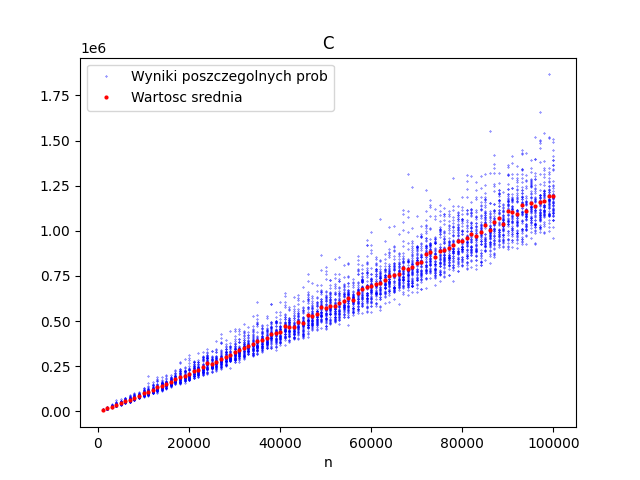
\includegraphics[scale=0.7]{plotC.png}
        \caption[Example .]{Wykres przedstawiający wyniki poszczególnych eksperymentów oraz wartość średnią \(C_{n}\)}
        \label{plotC}
    \end{figure}

    \begin{figure}[H]
        \centering
        \begin{subfigure}{.5\textwidth}
          \centering
          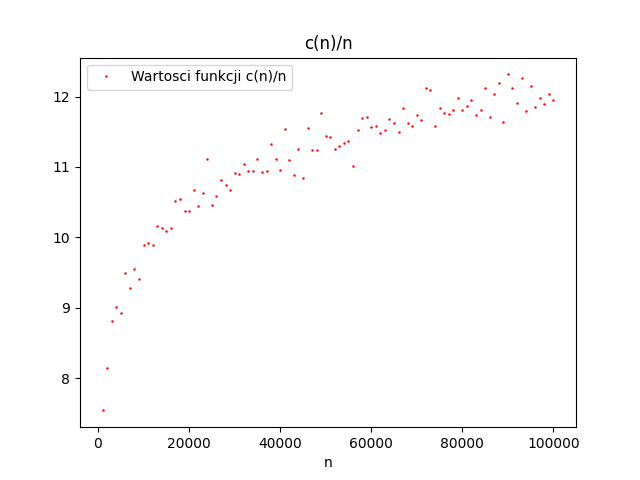
\includegraphics[width=1.1\linewidth]{plotcnfunc1.png}
          \caption{\( \frac{C_n}{n} \)}
          \label{fig:plotcnfunc1}
        \end{subfigure}%
        \begin{subfigure}{.5\textwidth}
          \centering
          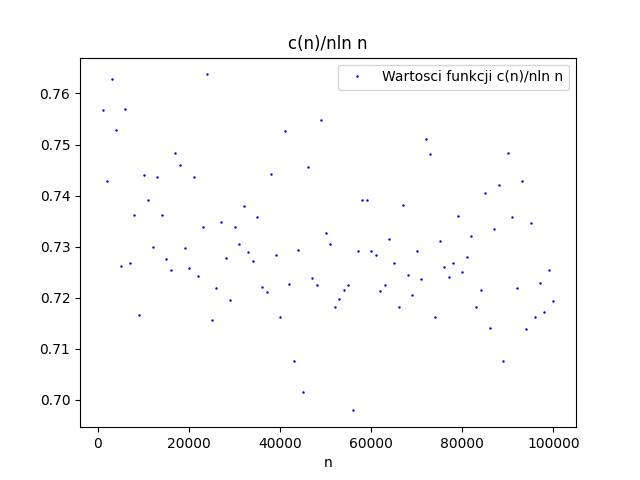
\includegraphics[width=1.1\linewidth]{plotcnfunc2.png}
          \caption{\( \frac{C_n}{nln(n)} \)}
          \label{fig:plotcnfunc2}
        \end{subfigure}
        \begin{subfigure}{.5\textwidth}
            \centering
            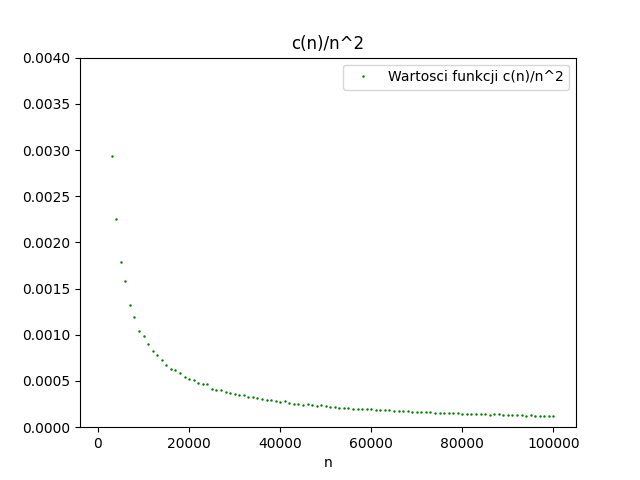
\includegraphics[width=1.2\linewidth]{plotcnfunc3.png}
            \caption{\( \frac{C_n}{n^2} \)}
            \label{fig:plotcnfunc3}
          \end{subfigure}
        \caption{Wykresy pomagające w znalezieniu asymptotyki funkcji \(C_n\)}
        \label{fig:cn}
    \end{figure}
    \center{Hipoteza:}
    \[C_n=O(nln(n))\]



\section*{Minimalna liczba rzutów, po której w kazdej z urn są co najmniej dwie kule \((D_n)\)}
\justifying
Tak jak wyżej koncetracja średniej początkowo jest dość silna, 
ale rośnie wraz z wartością \(n\).
\begin{figure}[htp]
        \centering
        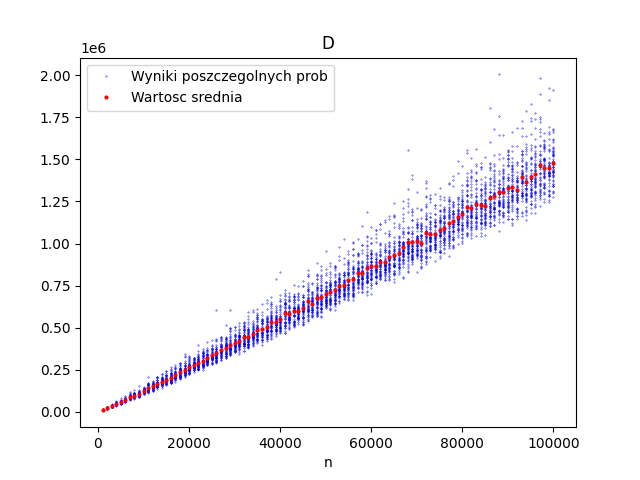
\includegraphics[scale=0.7]{plotD.png}
        \caption[Example .]{Wykres przedstawiający wyniki poszczególnych eksperymentów oraz wartość średnią \(D_{n}\)}
        \label{plotD}
    \end{figure}

    \begin{figure}[H]
        \centering
        \begin{subfigure}{.5\textwidth}
          \centering
          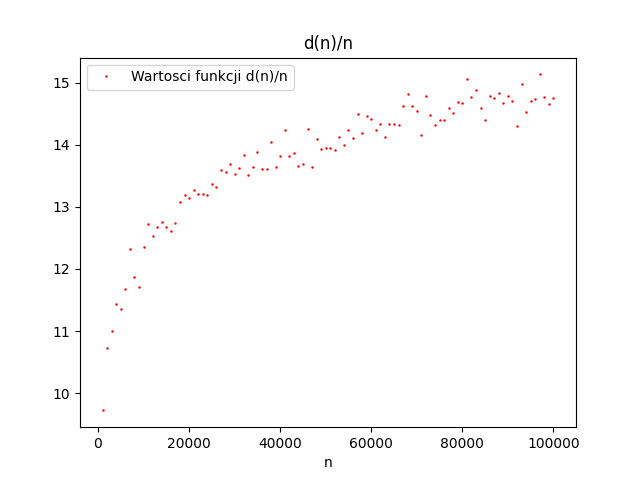
\includegraphics[width=1.1\linewidth]{plotdnfunc1.png}
          \caption{\( \frac{D_n}{n} \)}
          \label{fig:plotdnfunc1}
        \end{subfigure}%
        \begin{subfigure}{.5\textwidth}
          \centering
          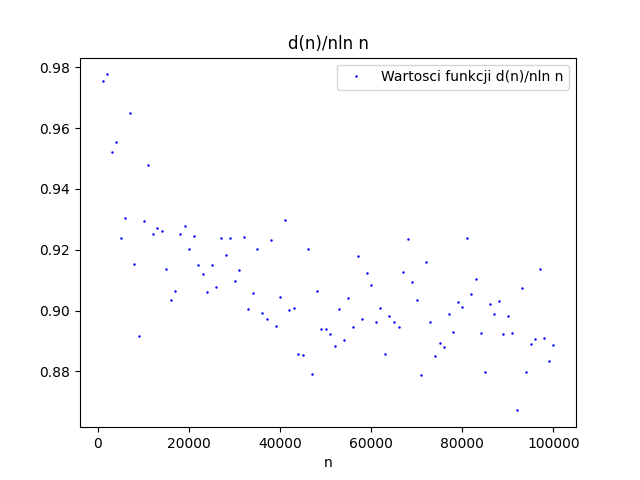
\includegraphics[width=1.1\linewidth]{plotdnfunc2.png}
          \caption{\( \frac{D_n}{nln(n)} \)}
          \label{fig:plotdnfunc2}
        \end{subfigure}
        \begin{subfigure}{.5\textwidth}
            \centering
            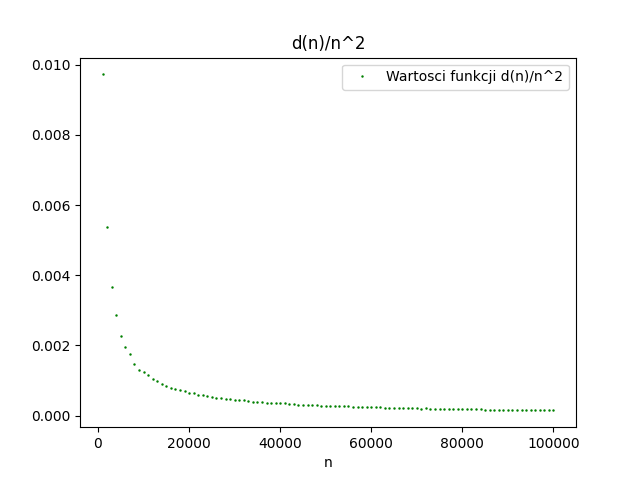
\includegraphics[width=1.2\linewidth]{plotdnfunc3.png}
            \caption{\( \frac{D_n}{n^2} \)}
            \label{fig:plotdnfunc3}
          \end{subfigure}
        \caption{Wykresy pomagające w znalezieniu asymptotyki funkcji \(D_n\)}
        \label{fig:dn}
    \end{figure}
    \center{Hipoteza:}
    \[D_n=O(nln(n))\]



\section*{Różnica \((D_n-C_n)\)}
\justifying
Ilość rzutów potrzebna do przejścia od momentu \(C_n\) do momentu \(D_n\).
Tutaj również koncentracja początkowo jest dość silna, ale przedział
przyjmowanych wartości bardzo szybko rośnie, więc koncentracja słabnie.
    \begin{figure}[htp]
        \centering
        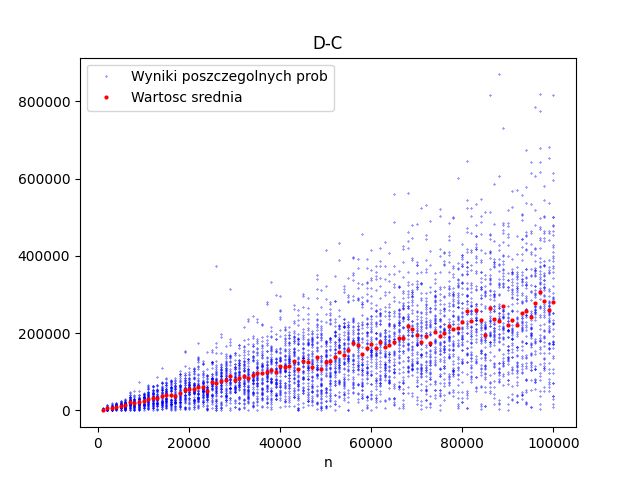
\includegraphics[scale=0.7]{plotD-C.png}
        \caption[Example .]{Wykres przedstawiający wyniki poszczególnych eksperymentów oraz wartość średnią \(D_{n}-C_{n}\)}
        \label{plotDC}
    \end{figure}

    \begin{figure}[H]
        \centering
        \begin{subfigure}{.5\textwidth}
          \centering
          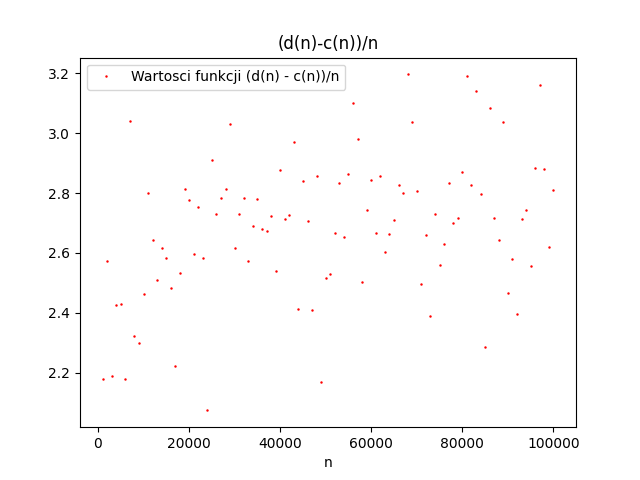
\includegraphics[width=1.1\linewidth]{plotdn-cnfunc1.png}
          \caption{\( \frac{D_n-C_n}{n} \)}
          \label{fig:plotdncnfunc1}
        \end{subfigure}%
        \begin{subfigure}{.5\textwidth}
          \centering
          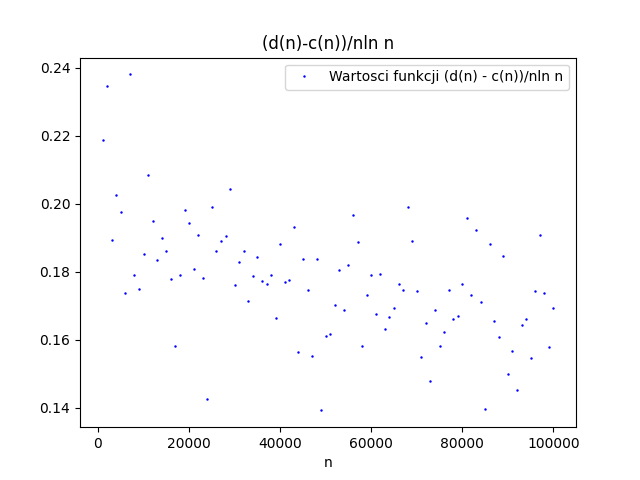
\includegraphics[width=1.1\linewidth]{plotdn-cnfunc2.png}
          \caption{\( \frac{D_n-C_n}{nln(n)} \)}
          \label{fig:plotdncnfunc2}
        \end{subfigure}
        \begin{subfigure}{.5\textwidth}
            \centering
            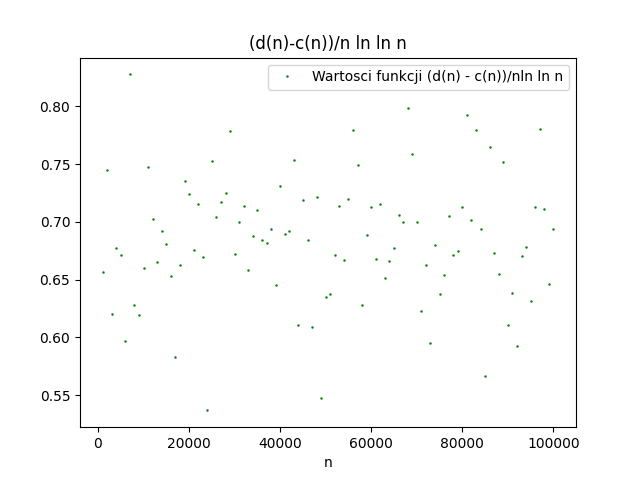
\includegraphics[width=1.2\linewidth]{plotdn-cnfunc3.png}
            \caption{\( \frac{D_n-C_n}{nln(ln(n))} \)}
            \label{fig:plotdncnfunc3}
          \end{subfigure}
        \caption{Wykresy pomagające w znalezieniu asymptotyki funkcji \(D_n-C_n\)}
        \label{fig:dncn}
    \end{figure}
\justifying
W tym konkrentym przypadku nasz sample size jest zbyt mały żeby określić asymptotykę
z samego wykresu. Obie funkcje \(D_n\) i \(C_n\) są asymptotyki \(O(nln(n))\) więc
\(D_n-C_n\leq O(nln(n))\), ale wszystkie funkcje przedstawione na wykresach również 
spełniają tę własność.
\[D_n-C_n=O(?)\]

\section*{Birthday paradox w kontekście funkcji hashujących}
\label{birthdayparadox}
Birthday paradox modeluje nam szansę, że nasz algorytm hashowania
stworzy dwa identyczne hashe dla dwóch różnych wejść. Przede wszystkim pokazuje on,
że pomimo tego, że nasza przestrzeń możliwych hashów jest duża, to szansa na to, że
generując je wielokrotnie, dwa będą takie same jest stosunkowo niewielka. W dodatku
maleje ona asymptotycznie do \(O(\sqrt{n})\), więc dość wolno.

\end{document}